\scanpage{86}

% top, lines 1–4
de $C^{*\circ}$. L'opposé de ce pavé \inserted{$\mathrm{Pav}(C)^\circ$} est can. isom \deleted{au pavé} \inserted{à} $\mathrm{Pav}(C^*)$, \deleted{\unsure{mais}} \unsure{Obtenu|Obtenir}, en \deleted{\unsure{notant que}} \deleted{\unsure{transformant de l'autre côté}}, \inserted{utilisant l'iso.} $\deleted{\unsure{\text{can}}}C^{**}\simeq C$ -- qui est l'isom can. composé avec l'antipodisme\ldots

% upper, display and annotations
\[
\mathrm{Pav}(\underset{\substack{\diagup\\\text{carré}\\\text{donné}}}{C})^\circ
\overset{\text{canon}}{\simeq}
\mathrm{Pav}(\underset{\substack{\diagup\\\text{carré dual de }C}}{C^*})
\]

% middle, NB
\uline{NB} Le produit des deux symétries de $X$ relatives aux triangles issus de $a$ est celui qui \deleted{échange entre eux les} \inserted{fixe $a$ et} induit l'antipodisme sur $C$ et sur $C^{*\circ}$

% middle-lower, universal property
$C\hookrightarrow\mathrm{Pav}(C)$ a la propriété universelle évidente pour les complexes trialitaires $\unsure{\mathcal X|\mathscr X}$ :

% lower, first display
\[
\mathrm{Pl}(\mathrm{Pav}(C),\mathcal X)\xrightarrow{\sim}\mathrm{Pl}(C,X)\qquad\text{(plongts)}
\]

% lower, next line
Si $\mathcal X$ est lui-$\overline{=}$ un pavé, on écrit

% lower, second display
\[
\mathrm{Iso}(\mathrm{Pav}(C),\mathcal X)\simeq\mathrm{Pl}(C,\mathcal X)
\]

% lower, final implication
Pour $\mathcal X$ complexe trialitaire donné, \deleted{\unsure{une}} la donnée d'un carré dans $\mathcal X$ revient à la donnée d'un \uline{pavé pointé} (car un carré est contenu dans un pavé unique\ldots)

% foot, NB and inline figure
\uline{NB} On fera attention que dans un graphe cubique un \uline{anticarré} (s'insérant \unsure{un.} dans un bitriangle
\figure{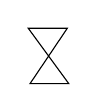
\begin{tikzpicture}[scale=.46]\draw (-.55,.77)--(.53,.77)--(-.5,-.76)--(.57,-.76)--cycle;\end{tikzpicture}}
) est contenu dans \uline{4} pavés

% archive sheet number: 85
